\chapter{各脏器增强影像特点}

腹部动态CT增强扫描是目前诊断腹部疾病的一种标准扫描模式,根据病灶的强化方式可以判断病变的良恶性、病变的范围等,因此了解腹部脏器的正常CT强化方式尤为重要,只有认识了正常的强化,才能使我们发现异常的强化,这对于发现腹部的各种疾病有十分重要的价值。本章我们将主要对腹部各个脏器在平扫时以及增强的不同时期的表现进行说明。

\section{各脏器强化值}

肝脏:平扫时肝实质CT值为55 Hu±10 Hu。

   动脉期肝实质强化不明显,CT值增加5~10 Hu。

   门静脉期肝实质明显强化,CT值为100 Hu±10 Hu。

脾脏:平扫时脾脏实质CT值为50 Hu±10 Hu。

   动脉期脾脏实质强化明显,CT值为95 Hu±10 Hu。

   门静脉期,脾脏实质CT值为100 Hu±10 Hu。

胰腺:平扫时胰腺实质CT值为45 Hu±5 Hu。

   动脉期胰腺实质中等强化,CT值为85 Hu±10 Hu。

   门静脉期,胰腺实质CT值为80 Hu±10 Hu。

肾脏:平扫时肾脏实质CT值为35 Hu±10 Hu。

   动脉期皮质明显强化,CT值为150 Hu±10 Hu。

   动脉期髓质强化较明显,CT值为60 Hu±10 Hu。

   静脉期皮质CT值为130 Hu±10 Hu。

   静脉期髓质强化较为明显,CT值为95 Hu±10 Hu。

\section{肝}

肝脏平扫时密度高于脾脏,且肝脏存在双重血供,即肝动脉及门静脉系统供血,且以门静脉供血所占比例高,因此门静脉期肝脏强化明显。

\begin{figure}[!htbp]
 \centering
 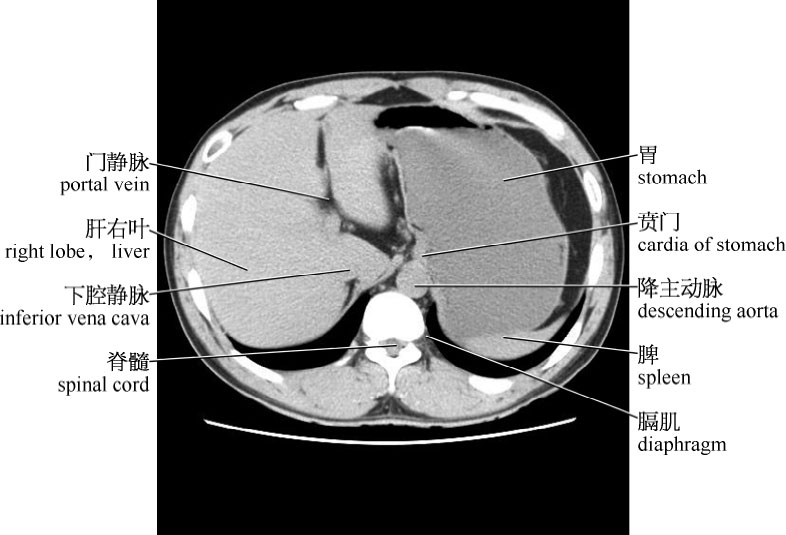
\includegraphics{./images/Image00140.jpg}
 \captionsetup{justification=centering}
 \caption{CT增强前}
  \end{figure} 
 \FloatBarrier

\begin{figure}[!htbp]
 \centering
 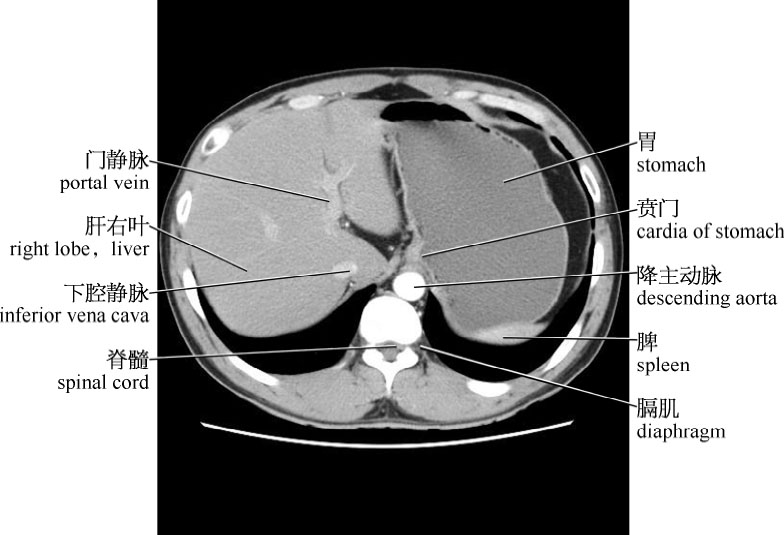
\includegraphics{./images/Image00141.jpg}
 \captionsetup{justification=centering}
 \caption{CT增强动脉期}
  \end{figure} 
 \FloatBarrier

\begin{figure}[!htbp]
 \centering
 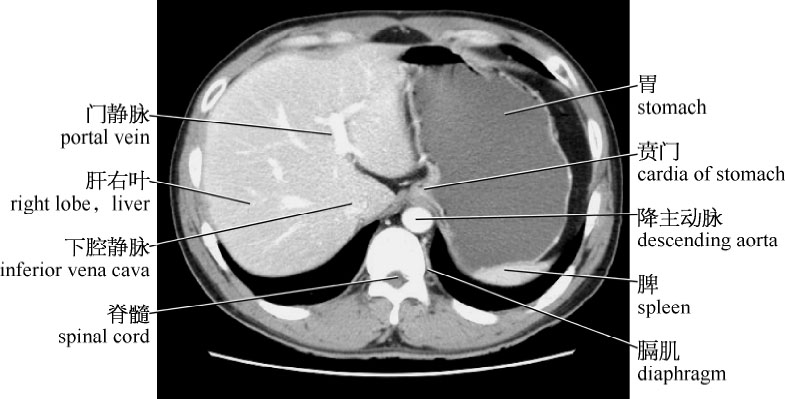
\includegraphics{./images/Image00142.jpg}
 \captionsetup{justification=centering}
 \caption{CT增强门静脉期}
  \end{figure} 
 \FloatBarrier

\section{脾 脏}

脾脏位于左上腹,平扫时密度略低于肝脏,脾脏血供较为丰富,因此强化明显。

\begin{figure}[!htbp]
 \centering
 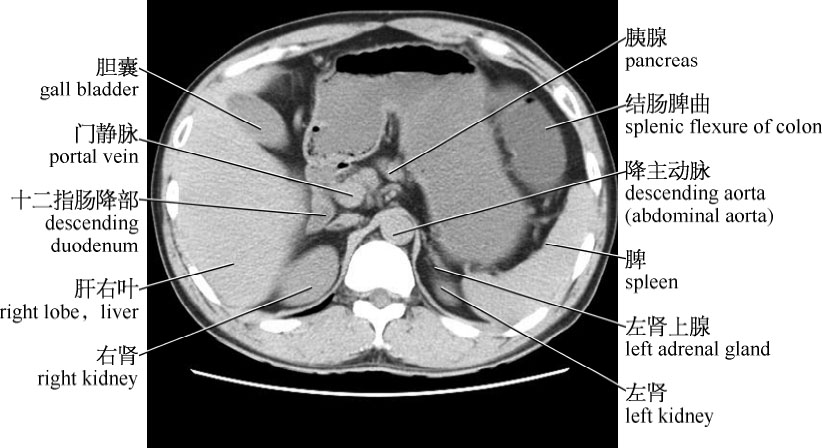
\includegraphics{./images/Image00143.jpg}
 \captionsetup{justification=centering}
 \caption{CT增强前}
  \end{figure} 
 \FloatBarrier

\begin{figure}[!htbp]
 \centering
 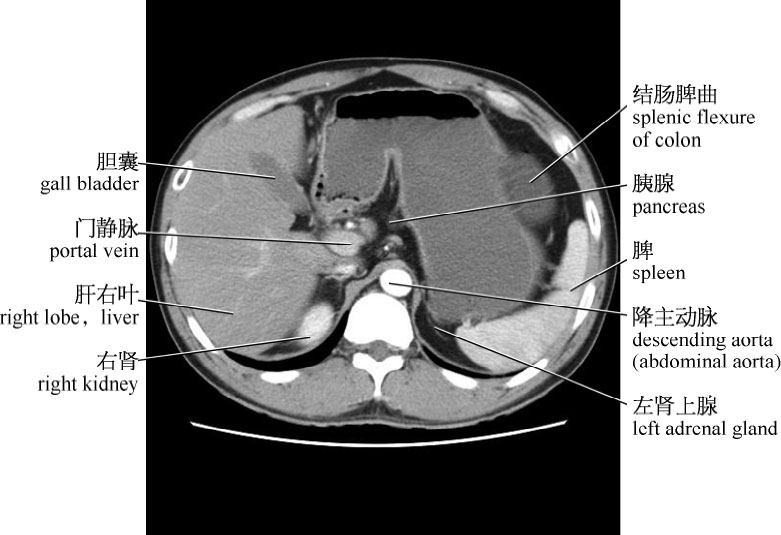
\includegraphics{./images/Image00144.jpg}
 \captionsetup{justification=centering}
 \caption{CT增强动脉期}
  \end{figure} 
 \FloatBarrier

\begin{figure}[!htbp]
 \centering
 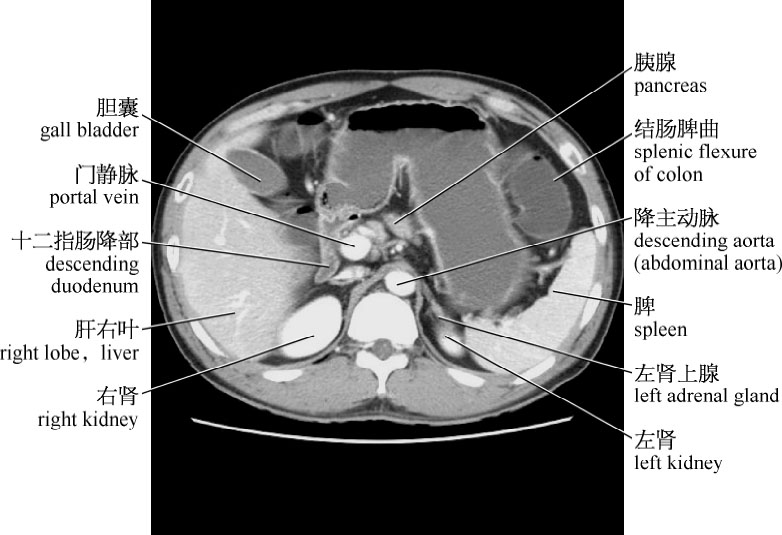
\includegraphics{./images/Image00145.jpg}
 \captionsetup{justification=centering}
 \caption{CT增强门静脉期}
  \end{figure} 
 \FloatBarrier

\section{胰 腺}

胰腺的血供较为丰富,但门静脉期胰腺实质的密度较动脉期降低。

\begin{figure}[!htbp]
 \centering
 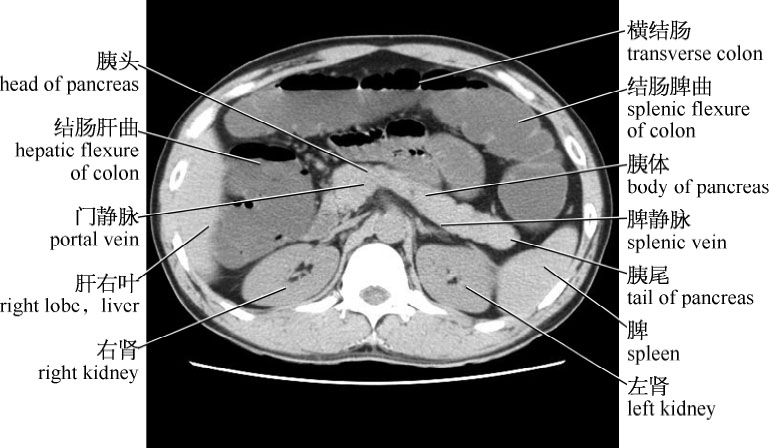
\includegraphics{./images/Image00146.jpg}
 \captionsetup{justification=centering}
 \caption{CT增强前}
  \end{figure} 
 \FloatBarrier

\begin{figure}[!htbp]
 \centering
 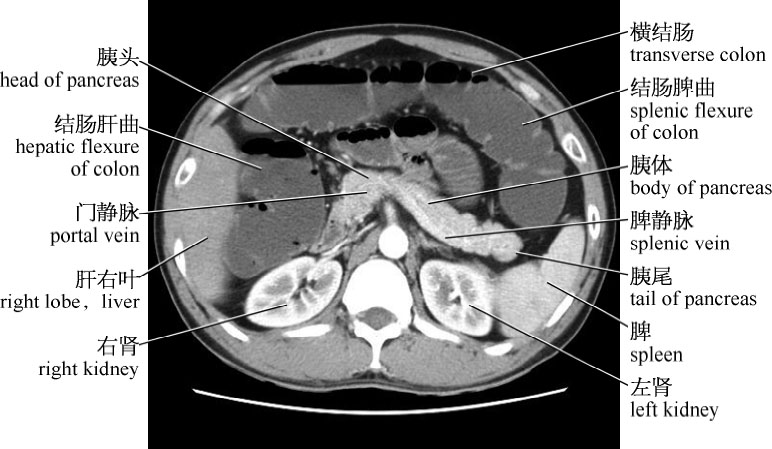
\includegraphics{./images/Image00147.jpg}
 \captionsetup{justification=centering}
 \caption{CT增强动脉期}
  \end{figure} 
 \FloatBarrier

\begin{figure}[!htbp]
 \centering
 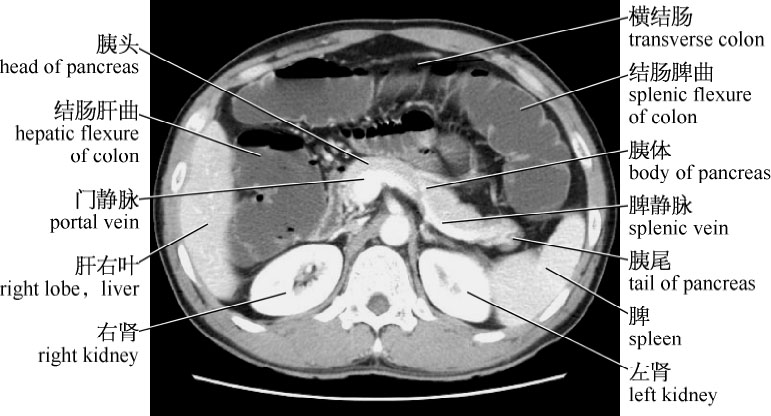
\includegraphics{./images/Image00148.jpg}
 \captionsetup{justification=centering}
 \caption{CT增强门静脉期}
  \end{figure} 
 \FloatBarrier

\section{消化道}

消化道为一空腔结构,消化道的管壁于门静脉期可出现较为明显强化。

\begin{figure}[!htbp]
 \centering
 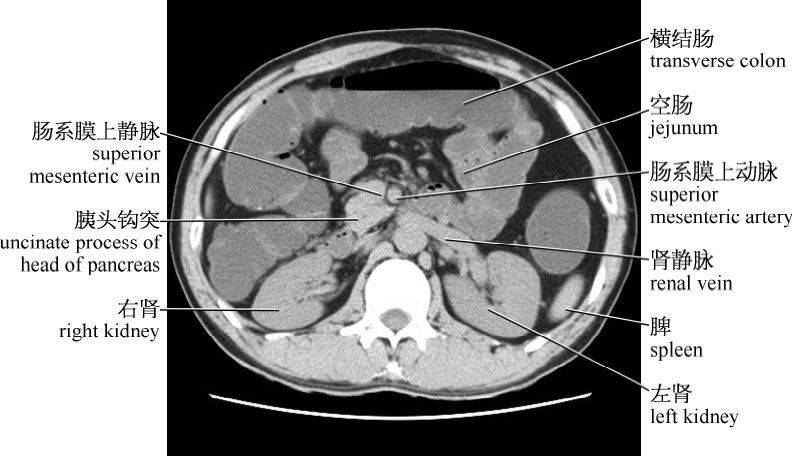
\includegraphics{./images/Image00149.jpg}
 \captionsetup{justification=centering}
 \caption{CT增强前}
  \end{figure} 
 \FloatBarrier

\begin{figure}[!htbp]
 \centering
 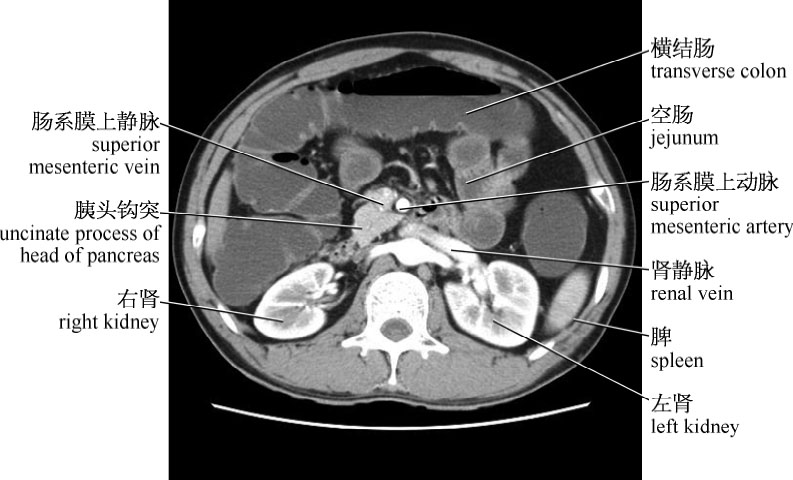
\includegraphics{./images/Image00150.jpg}
 \captionsetup{justification=centering}
 \caption{CT增强动脉期}
  \end{figure} 
 \FloatBarrier

\begin{figure}[!htbp]
 \centering
 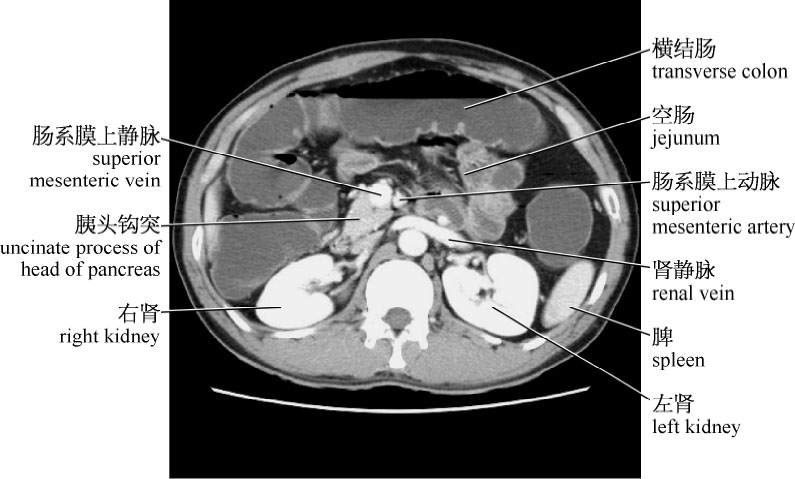
\includegraphics{./images/Image00151.jpg}
 \captionsetup{justification=centering}
 \caption{CT增强门静脉期}
  \end{figure} 
 \FloatBarrier

\section{肾 脏}

肾脏血供丰富,动脉期可出现明显肾皮质强化,至门静脉期肾脏髓质亦可出现较为明显的增强。

\begin{figure}[!htbp]
 \centering
 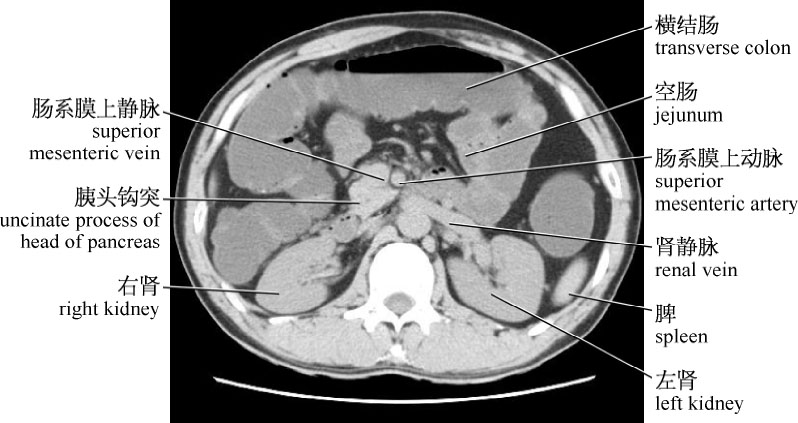
\includegraphics{./images/Image00152.jpg}
 \captionsetup{justification=centering}
 \caption{CT增强前}
  \end{figure} 
 \FloatBarrier

\begin{figure}[!htbp]
 \centering
 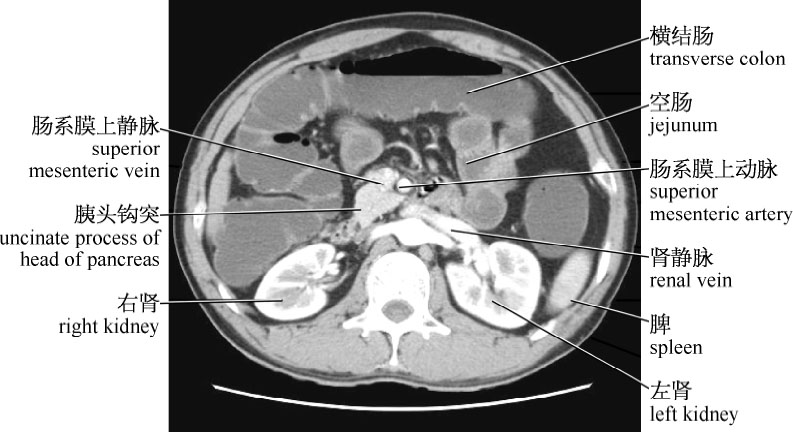
\includegraphics{./images/Image00153.jpg}
 \captionsetup{justification=centering}
 \caption{CT增强动脉期}
  \end{figure} 
 \FloatBarrier

\begin{figure}[!htbp]
 \centering
 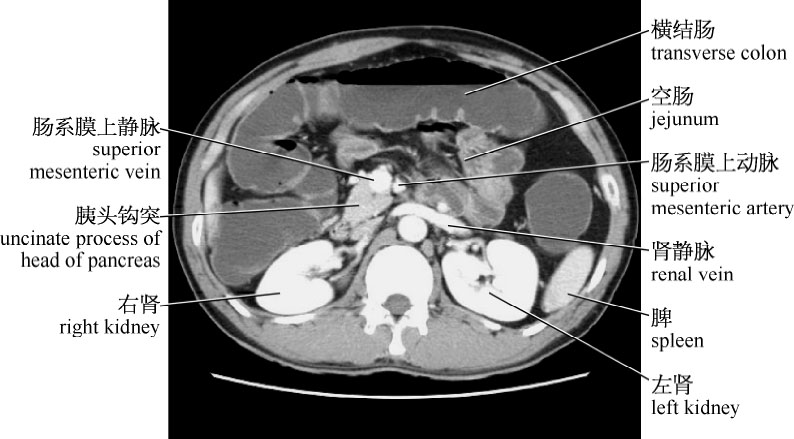
\includegraphics{./images/Image00154.jpg}
 \captionsetup{justification=centering}
 \caption{CT增强门静脉期}
  \end{figure} 
 \FloatBarrier

\section{膀 胱}

膀胱为储存,浓缩尿液的器官,充满尿液时显示清晰,膀胱壁存在一定的强化。

\begin{figure}[!htbp]
 \centering
 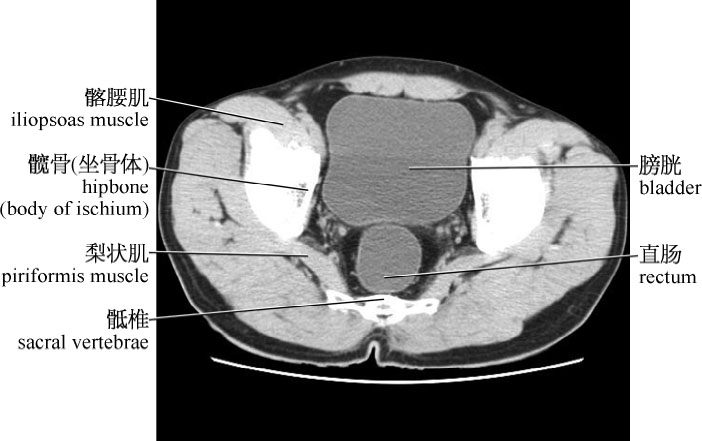
\includegraphics{./images/Image00155.jpg}
 \captionsetup{justification=centering}
 \caption{CT增强前}
  \end{figure} 
 \FloatBarrier

\begin{figure}[!htbp]
 \centering
 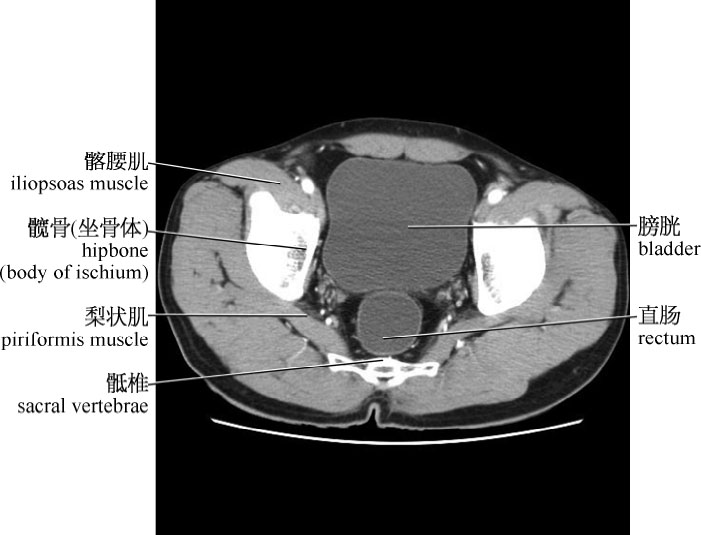
\includegraphics{./images/Image00156.jpg}
 \captionsetup{justification=centering}
 \caption{CT增强动脉期}
  \end{figure} 
 \FloatBarrier

\begin{figure}[!htbp]
 \centering
 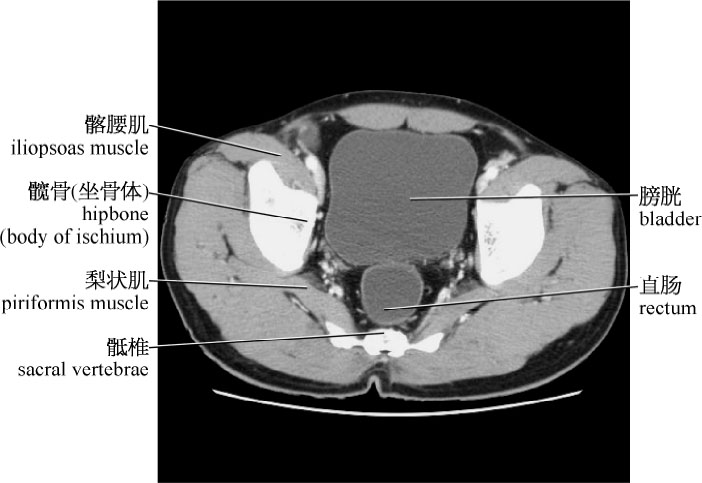
\includegraphics{./images/Image00157.jpg}
 \captionsetup{justification=centering}
 \caption{CT增强门静脉期}
  \end{figure} 
 \FloatBarrier

\section{子 宫}

子宫血供丰富,增强后子宫内膜可以出现较为明显强化。

\begin{figure}[!htbp]
 \centering
 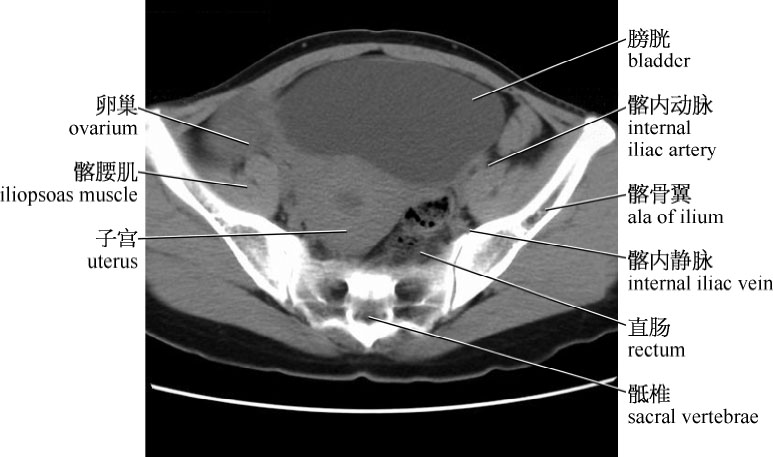
\includegraphics{./images/Image00158.jpg}
 \captionsetup{justification=centering}
 \caption{CT增强前}
  \end{figure} 
 \FloatBarrier

\begin{figure}[!htbp]
 \centering
 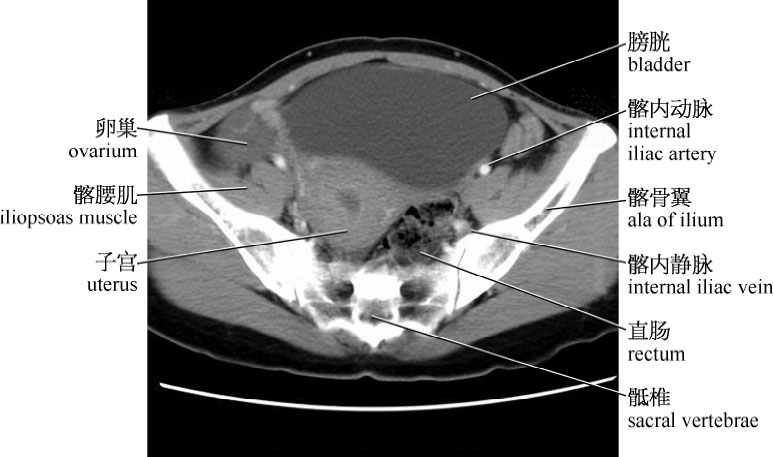
\includegraphics{./images/Image00159.jpg}
 \captionsetup{justification=centering}
 \caption{CT增强动脉期}
  \end{figure} 
 \FloatBarrier

\begin{figure}[!htbp]
 \centering
 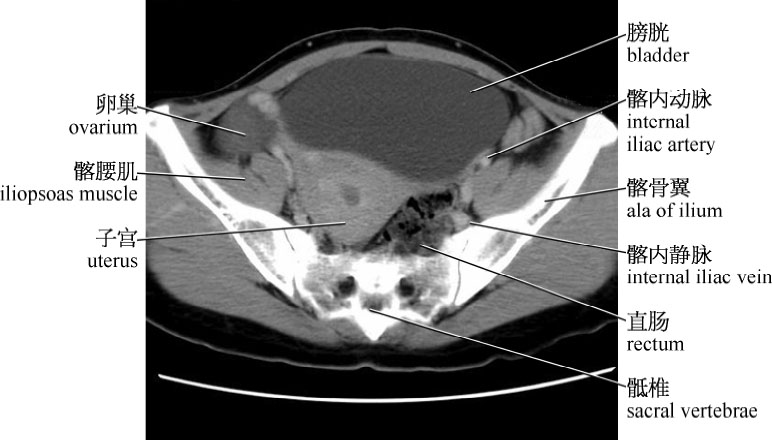
\includegraphics{./images/Image00160.jpg}
 \captionsetup{justification=centering}
 \caption{CT增强门静脉期}
  \end{figure} 
 \FloatBarrier

\section{前列腺}

前列腺为男性生殖系统的一个重要组成部分,增强后可以出现一定增强。

\begin{figure}[!htbp]
 \centering
 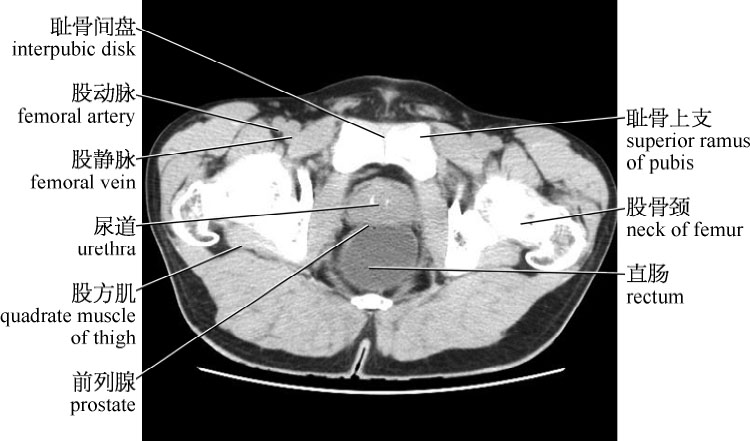
\includegraphics{./images/Image00161.jpg}
 \captionsetup{justification=centering}
 \caption{CT增强前}
  \end{figure} 
 \FloatBarrier

\begin{figure}[!htbp]
 \centering
 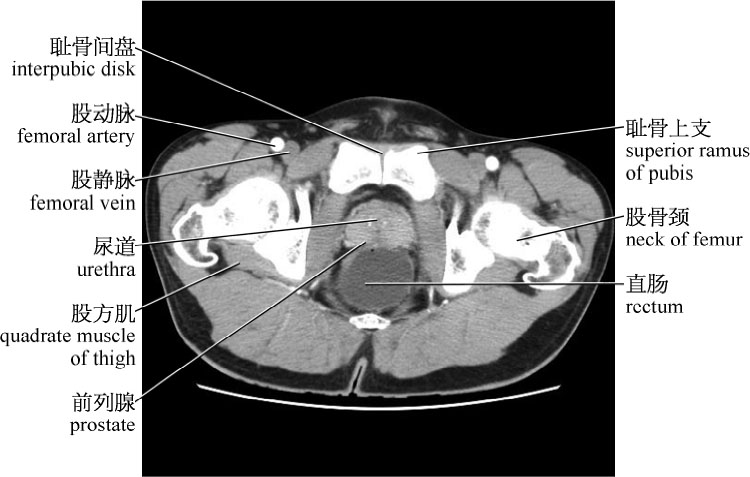
\includegraphics{./images/Image00162.jpg}
 \captionsetup{justification=centering}
 \caption{CT增强动脉期}
  \end{figure} 
 \FloatBarrier

\begin{figure}[!htbp]
 \centering
 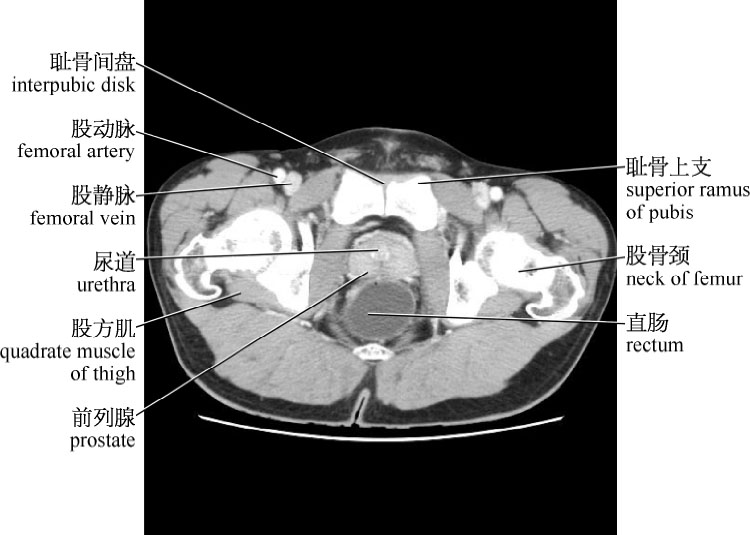
\includegraphics{./images/Image00163.jpg}
 \captionsetup{justification=centering}
 \caption{CT增强门静脉期}
  \end{figure} 
 \FloatBarrier
